
%(BEGIN_QUESTION)
% Copyright 2014, Tony R. Kuphaldt, released under the Creative Commons Attribution License (v 1.0)
% This means you may do almost anything with this work of mine, so long as you give me proper credit

When the 5 k$\Omega$ potentiometer in this circuit is set to its 0\%, 25\%, 50\%, 75\%, and 100\% positions, the following output voltages are obtained (measured with respect to ground, of course):

$$\includegraphics[width=15.5cm]{i01132x01.eps}$$

\begin{itemize}
\item{} At 0\% setting, $V_{out} = 0 \hbox{ V}$
\item{} At 25\% setting, $V_{out} = 2.5 \hbox{ V}$
\item{} At 50\% setting, $V_{out} = 5 \hbox{ V}$
\item{} At 75\% setting, $V_{out} = 7.5 \hbox{ V}$
\item{} At 100\% setting, $V_{out} = 10 \hbox{ V}$
\end{itemize}

Calculate what the output voltages will be if a 1 k$\Omega$ load resistor is connected between the ``$V_{out}$'' terminal and ground:

$$\includegraphics[width=15.5cm]{i01132x02.eps}$$

\begin{itemize}
\item{} At 0\% setting, $V_{out} = $
\item{} At 25\% setting, $V_{out} = $
\item{} At 50\% setting, $V_{out} = $
\item{} At 75\% setting, $V_{out} = $
\item{} At 100\% setting, $V_{out} = $
\end{itemize}

\underbar{file i01132}
%(END_QUESTION)





%(BEGIN_ANSWER)
\begin{itemize}
\item{} At 0\% setting, $V_{out} = 0 \hbox{ V}$
\item{} At 25\% setting, $V_{out} = 1.29 \hbox{ V}$
\item{} At 50\% setting, $V_{out} = 2.22 \hbox{ V}$
\item{} At 75\% setting, $V_{out} = 3.87 \hbox{ V}$
\item{} At 100\% setting, $V_{out} = 10 \hbox{ V}$
\end{itemize}
%(END_ANSWER)





%(BEGIN_NOTES)

This question is really nothing more than five loaded voltage divider problems packed into one!  It is a very practical question, as potentiometers are very often used as variable voltage dividers, and students must realize the effects a load resistance will have on the characteristics of such dividers.  Point out to them the extreme nonlinearity created by the inclusion of the load resistance.

%INDEX% Electronics review: series-parallel circuits

%(END_NOTES)


